\section{Measurement Strategy}\label{s:measurement}

In this section we describe how the \inbox and \outbox coordinate to compute accurate and robust
measurements of the network conditions necessary as inputs to congestion control algorithms.

Congestion control algorithms need only a small, common set of measurements~\cite{ccp-hotnets}. 
In particular, rate-based algorithms need only three measurements: 
the sending rate, receiving rate, and path round-trip time.
A significant complication is that for accurate measurements on RTT time-scales, we must calculate send and receive rates over the same set of packets~\cite{packettrain} \radhika{one line explanation on why}.
This requirement drives the design of our measurement methodology.

\subsection{Determining Epoch Boundary Packets}
\label{s:measure:marking}
Consider the stream of packets $P_B$ from all flows in a bundle $B$ in the order they leave the \inbox after scheduling.
The \inbox and \outbox need to know how to divide this stream into sets 
of packets --- which we call \emph{epochs} --- over which they can calculate measurements.
For now, we make the simplifying assumption that packets arrive at the \outbox in the same order they 
left the \inbox\footnote{We address re-ordering in Section~\ref{s:measure:limitation:reorder}}.
This simplifies the problem into deciding, for all given packets in $P_B$, whether it is an epoch boundary packet at which the current epoch should end and the next should begin. 
Suppose for now that we wish to have a fixed epoch size of $N$ packets.
A naive approach would be to mark the boundary between epochs every $N$ packets. 
However, this strategy is brittle; a single lost packet would de-synchronize the boxes' views of the epochs. 
More generally, any strategy that requires packet-level synchronization of the \inbox and
\outbox is untenable because any coordination would race the packets themselves \radhika{i don't quite understand the last sentence}.

The key idea of our methodology is that we can avoid such a synchronization problem by determining the boundary of an epoch using only information contained in the packet.
Specifically, we propose the following: a packet $p$ is an epoch boundary packet if the hash 
of some subset of its header (see below) modulo the epoch size $N$ is equal to 0, that is:
$$B(p,N) \coloneqq H(p)\ \text{mod}\ N == 0$$
\radhika{equation not super clear}
Thus, an epoch boundary packet will occur (in expectation) once every $N$ packets.
For $H$, we use the Fowler/Noll/Vo (FNV) hash function~\cite{fnv-hash}, a non-cryptographic fast hash function with a low collision rate. 

\paragrapha{Choosing header subset} The header subset we use must remain constant as the packet traverses the network from the \inbox to the \outbox; otherwise, they would not be able to agree on epoch boundaries. This rules out simple approaches such as hashing the entire packet header, since the TTL field will decrement between the inbox and outbox.
Even the 5-tuple of the packet may change, since the outbox may be behind a NAT.
Using TCP sequence numbers is tempting, but retransmissions may confuse RTT measurements.

We use the IP ID field, which will change every packet. This is an imperfect solution, as modern NATs may rewrite the IP ID field~\cite{ipid}.
Ultimately, the appropriate field to use will depend on the specific deployment of \name. \fc{come back to this, mention boxes are not likely to be behind NATs therefore you can do ipid+5tuple }

\subsection{Computing Measurements}
\label{s:measure:compute}
\newcommand{\pone}{$p_{prev}$}
\newcommand{\hpone}{$h(p_{prev})$}
\newcommand{\sone}{$s_{prev}$}
\newcommand{\rone}{$r_{prev}$}
\newcommand{\ptwo}{$p_{curr}$}
\newcommand{\hptwo}{$h(p_{curr})$}
\newcommand{\stwo}{$s_{curr}$}
\newcommand{\rtwo}{$r_{curr}$}
\newcommand{\atwo}{$a_{curr}$}
\newcommand{\sentone}{$sent_{prev}$}
\newcommand{\recvdone}{$rcvd_{prev}$}
\newcommand{\senttwo}{$sent_{curr}$}
\newcommand{\recvdtwo}{$rcvd_{curr}$}


\begin{figure}
    \centering
    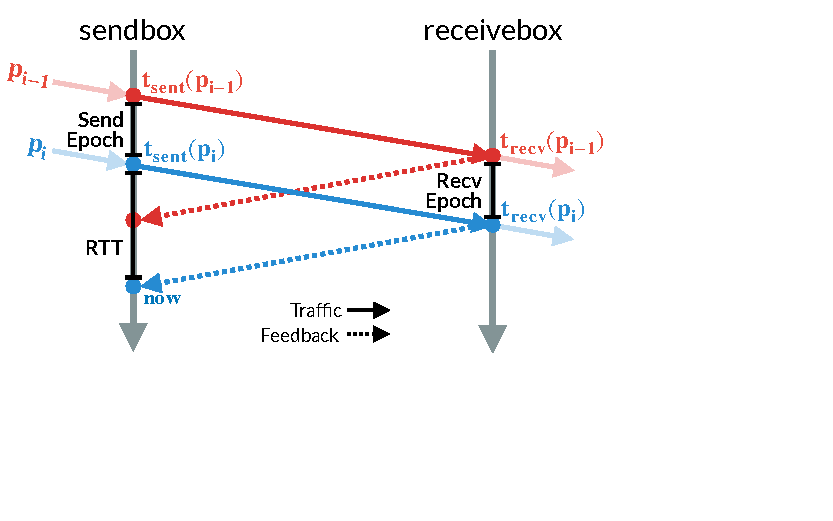
\includegraphics[width=\columnwidth]{img/rate-calculation}
    \caption{Example of epoch-based measurement calculation. Time moves from top to bottom.
    Packets from flows in a bundle
    pass through the \inbox and \outbox middleboxes on the way to their destination. When 
    the inbox observes a packet header matching the boundary condition, it records it. When
    the \outbox observes such a packet, it sends an out-of-band feedback message back to
    the \inbox, which allows it to calculate the RTT and epochs.}\label{fig:ratecalc}
\end{figure}

Given this method of marking epochs, we can now construct the procedure for computing measurements.

For a given bundle, the \inbox runs the aforementioned function on each packet $p$. Each time
the function returns true, the \inbox updates an epoch data structure that records the packet hash,
which we will call \hptwo\ for the current epoch, 
along with the current time \stwo\ and the \emph{cumulative} number of bytes sent so far, \senttwo. This structure
is sorted by the time the packet was sent, \stwo, but is indexable by the packet hash.

The \outbox runs the same function. Each time it observes a boundary packet, 
it immediately sends a feedback message to the \inbox containing the same information:
the packet hash \hptwo, the time at which it received the packet, \rtwo, and the cumulative number of bytes
\emph{received} up until that point. When the \inbox receives this feedback message at time \atwo, it looks up the
packet hash \hptwo\ in the epoch data structure, which represents the end of the current epoch,
along with the earliest boundary packet still in the data structure, \hpone\ which represents the start
of the current epoch. It now has all of the information necessary to calculate one sample of the following:
\begin{subequations}
    \begin{align}
        RTT &= &now - s_2 \\
        send\_epoch\_duration &= &s_2 - s_1\\
        recv\_epoch\_duration &= &r_2 - r_1\\
        bytes\_sent\_in\_epoch &= &bytes\_sent\ at\ s_2 &\ - \\
                                    &&bytes\_sent\ at\ s_1&\notag\\
        bytes\_rcvd\_in\_epoch &= &bytes\_rcvd\ at\ r_2 &\ - \\
                                &&bytes\_rcvd\ at\ r_1\notag\\
        send\_rate &= &\frac{bytes\_sent\_in\_epoch}{send\_epoch\_duration}\\
        recv\_rate &= &\frac{bytes\_rcvd\_in\_epoch}{recv\_epoch\_duration}
    \end{align}
\end{subequations}
%(Note $bytes\_rcvd\_in\_epoch$ can also be interpreted as the number of bytes
%acknowledged for that epoch, which is a common signal used by many conestion
%control algorithms.)
Finally, it clears all marked packets preceding \ptwo\ leaving \ptwo\
to be the start of the next epoch.

\subsection{Fault Tolerance}
\label{s:measure:loss}
\paragrapha{Packet loss} This method is robust to the loss of boundary packets between the \inbox and \outbox.
Suppose the \inbox sees boundary packets $p_1, p_2, p_3$, but $p_2$ is lost after passing through
the \inbox so the \inbox only receives feedback for $p_1$ and $p_3$. Upon receiving $p_1$, 
the \inbox will truncate its data structure up until $p_1$. Upon receiving $p_3$, the \inbox 
looks up the oldest remaining boundary packet, $p_1$, and considers that the beginning of the epoch.
As a result, the epoch is longer than expected, but no measurements are lost or corrupted. 
The same argument applies to the loss of feedback messages. 
Importantly, \inbox calculates both the send and receive epoch based on information
from the \outbox rather than attempting to reach consensus on individual epoch boundaries with the \outbox. 

% \paragrapha{Crashes \an{need better heading}} Existing work~\cite{ftmb} has studied how to design stateful middleboxes to be fault-tolerant with acceptable performance overheads. 
% However, state-persistence is largely unnecessary for \name.
% \name only stores network conditions, which it can re-learn within a few RTTs, and bundle membership flow tables, which it can re-discover as we describe in~\S\ref{s:impl:discovery}. 
% \radhika{maybe move elsewhere}

\subsection{Choosing The Epoch Size}
\label{s:measure:epoch}
\begin{figure}
    \centering
\begin{knitrout}
\definecolor{shadecolor}{rgb}{0.969, 0.969, 0.969}\color{fgcolor}
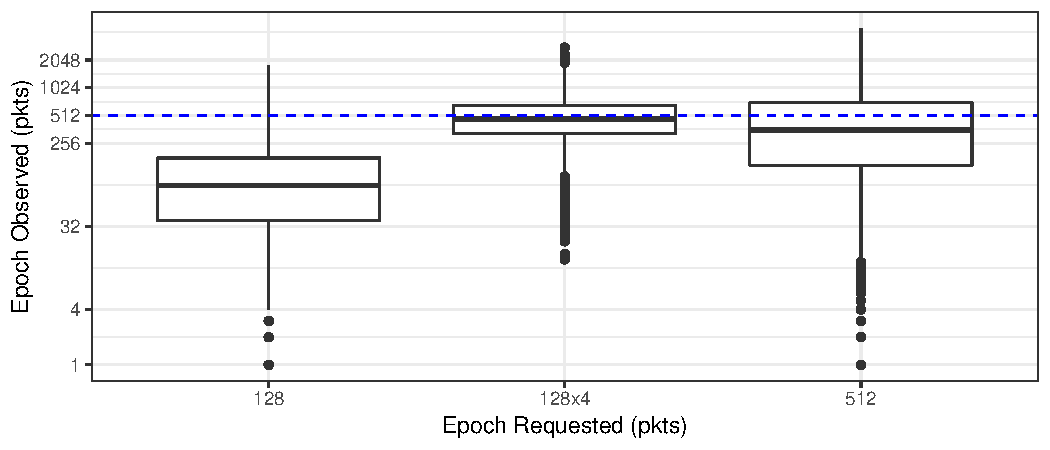
\includegraphics[width=\maxwidth]{figure/micro:epoch-1} 

\end{knitrout}
    \caption{Distribution of observed epoch sizes based on the desired epoch size. Suppose we
    need an epoch size of 512. By setting the epoch size to $\frac{1}{4}$ of that and using
    a sliding window over the last 4 epochs, we can achieve the same average epoch size with
    significantly lower variance than if we were to set the epoch size to 512 directly.
    \fc{todo: real eval data}}
    \label{fig:micro:epoch}
\end{figure}


How do we choose the number of packets that should be in each epoch?
In \S\ref{s:measure:marking}, we assumed a fixed epoch size of $N$ packets.
However, in practice, the epoch must be a function of the bandwidth-delay product (BDP).
Because epoch sizes are sampled from a uniform random variable, setting larger epoch sizes will increase the variance in the observed epoch sizes.
If the epoch size is small relative to the rate, the raw measurements will be noisy, but we can correct for this by measuring over a sliding window.

Therefore, we estimate the BDP (current sending rate multiplied by current estimate of the RTT) and set the desired epoch size to one-fourth of this value. We then calculate rates over a sliding window of four epochs; this is approximately one RTT.

As the sending rate and RTT change, the \inbox will update the desired epoch size accordingly, and communicate this desired epoch size to the \outbox.
This communication might be lost. 
Therefore, when setting the desired epoch size we round down to the nearest power of two so that the \outbox's view of the epoch boundary packets is a sub- or super- set of the \inbox's:
for example, 
if the \inbox's desired epoch size is $64$ packets
but the \outbox does not receive this update and still believes the desired epoch size is $128$ packets, 
the \outbox's feedback will still match (in expectation) half the \inbox's epoch boundary packets.

\subsection{Microbenchmarks}
\label{s:measure:microbench}
    \begin{figure}
    \centering
\begin{knitrout}
\definecolor{shadecolor}{rgb}{0.969, 0.969, 0.969}\color{fgcolor}
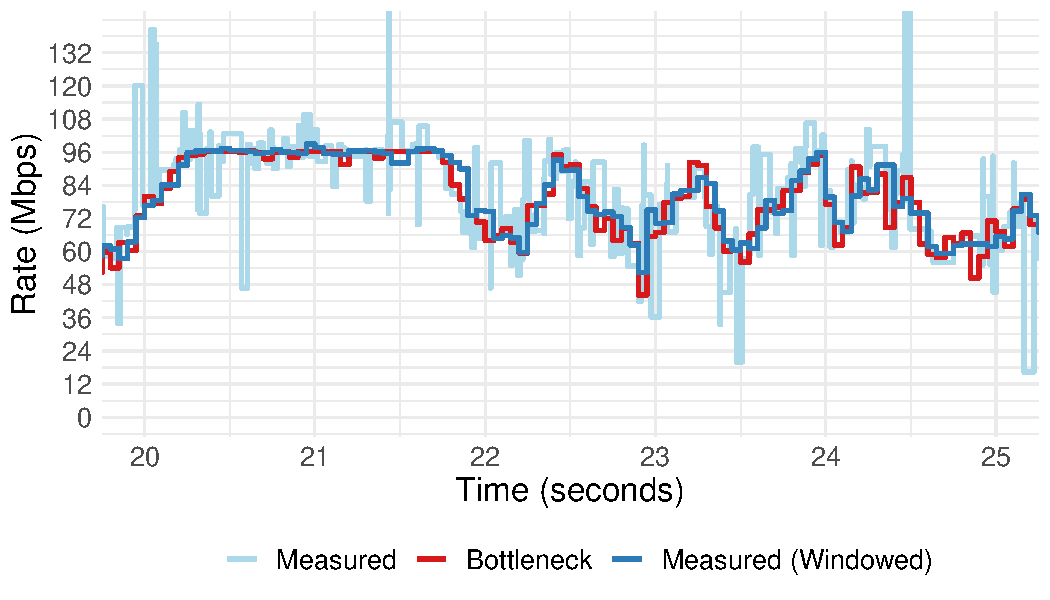
\includegraphics[width=\maxwidth]{figure/micro:time-1} 

\end{knitrout}
    \caption{\name's estimate of the receive rate compared to the actual rate leaving the bottleneck over a five second trace. 
    \name's raw estimate of the rate hovers around the true value, but is noisy. Averaging over a window of previous epochs
    yields a much smoother estimate that closely matches the true value.}
    \label{fig:micro:time}
\end{figure}

    \begin{figure}
    \centering
\begin{knitrout}
\definecolor{shadecolor}{rgb}{0.969, 0.969, 0.969}\color{fgcolor}
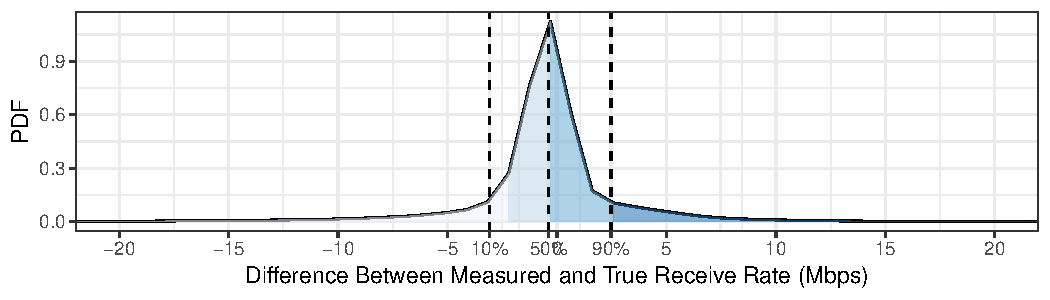
\includegraphics[width=\maxwidth]{figure/micro:thru-1} 

\end{knitrout}
    \caption{Distribution of the difference between \name's smoothed estimate of the receive rate and 
    the true bottleneck rate at each time point across all experiments. In most cases, the difference
    is negligble.}
    \label{fig:micro:thru}
\end{figure}

    \begin{figure}
    \centering
\begin{knitrout}
\definecolor{shadecolor}{rgb}{0.969, 0.969, 0.969}\color{fgcolor}
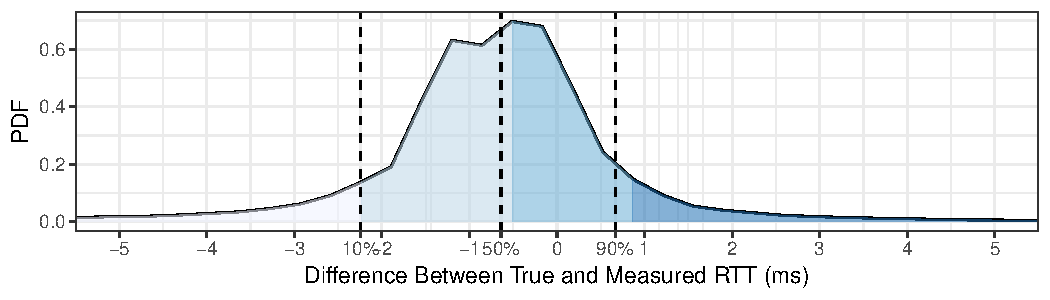
\includegraphics[width=\maxwidth]{figure/micro:delay-1} 

\end{knitrout}
    \caption{Distribution of the difference between \name's smoothed estimate of the RTT and 
    the true RTT (based on the queueing delay at the bottleneck router) at each time point across all experiments. In most cases, the difference
    is negligble.}
    \label{fig:micro:delay}
\end{figure}

    In this section we explore how well our measurements match the actual network conditions. 

    First, we consider our estimate of the receive rate (via Equation 1g). In Figure~\ref{fig:micro:time}
    we compare our esimate of the receive rate (``Measured'') to the actual rate of packets 
    leaving the bottleneck over a five second segment from one run in our evaluation (\fc{expand}).
    Here we demonstrate the necessity of a window to smooth out the estimation.

    In Figure~\ref{fig:micro:thru}, we compute the difference between our smoothed estimate of the receive rate 
    and the bottleneck rate at each time step and plot the distribution of this difference across
    all of the traces in our evaluation. 80\% of the time our estimate is within 3Mbps of the 
    actual rate.

    In Figure~\ref{fig:micro:delay}, we compute the difference between our estimate of the RTT between
    the \inbox and \outbox and the actual RTT at each time stpe and plot the distribution again
    across all of the traces in our evaluation. 80\% of the time we are within 2ms of the actual RTT.
    \radhika{discuss}
    
\subsection{Limitations}
\subsubsection{Re-Ordering}
\label{s:measure:limitation:reorder}
Earlier we ignored re-ordering of packets between the \inbox and \outbox. However, if packets
are re-ordered, the \inbox and \outbox will observe a different view of the same epoch.
For example, consider packets numbered 1 to 20, where 10 is a boundary packet. The \inbox observes
10 packets in each epoch: [1,10] in epoch 1 and [11,20] in epoch 2. 
However, suppose packet 7 is delayed and arrives after packet 10. The \outbox will observe 9
packets in epoch 1 and 11 packets in epoch 2. 
Spurious re-ordering can be compensated by using an EWMA across epochs rather than the raw values
calculated at each epoch. If there is persitent re-ordering, it may be necessary to add a constant 
value to either the send or receive rate to compensate.
\radhika{the explanation seems a bit hand-wavy. if we end up doing ecmp expt and the results look good, add fwd pointer to those results}

\subsubsection{Suitable Algorithms}
\label{s:measure:limitation:algs}
The set of measurements we obtain are sufficient for most rate-based algorithms, but may not be 
suitable for traditional window-based algorithms which require low-level metrics such as 
the number of inflight packets or number of packets lost. Although it should be possible
to compute these from the measurements we already collect in an ideal scenario, they would easily
break in the presence of network anomilies such as re-ordering. Thus, we leave the development
of robust signals for window-based algorithms to fuure work. 
Thus, \name currently operates best with rate-based algorithms such as BBR, Nimbus, or Copa~\cite{bbr,nimbus,copa}.
\radhika{feels like this should be moved to Sec 3, but am  not entirely sure.}
